\documentclass[10pt, draft]{book}


\usepackage[latin1]{inputenc}
\usepackage[T1]{fontenc}
\usepackage[italian]{babel}
\usepackage{a4wide}
\usepackage{makeidx}
\usepackage{url}
\usepackage{multicol}
\usepackage{amsthm}
\usepackage{colortbl}
\usepackage{amssymb}
\usepackage{synttree}
\usepackage{proof}


\newtheorem{teorema}{Teorema}
\newtheorem{proposizione}{Proposizione}
\newtheorem{corollario}{Corollario}
\newtheorem{definizione}{Definizione}
\newtheorem{osservazione}{Osservazione}
\newtheorem{notazione}{Notazione}
\newtheorem{lemma}{Lemma}
\newtheorem{esempio}{Esempio}
\newtheorem{dimostrazione}{Dimostrazione}

\title{Backend\\[2mm]{\small\emph{Anno Accademico 2010-2011}}\\[4mm]}
\author{\Nome\ \Cognome}

\newcommand{\Cognome}{Viscomi}
\newcommand{\Nome}{Federico}



\makeindex

\begin{document}

\maketitle

\tableofcontents

\chapter{Introduzione}
Questo documento descrive:
\begin{itemize}
  \item 
    La struttura composita della parte del backend che gestisce una singola partita. Per una descrizione del resto del backend si faccia riferimento al documento architettura\_e\_design.pdf
  \item
    Le varie iterazioni del processo di sviluppo che ha portato all'implementazione del backend.
  \item
    Come e' stato testato il backend.
\end{itemize}


\chapter{Struttura del backend}
La figura 1 descrive la struttura composita di una certa porzione di Cupido. I

\begin{center}
  \begin{figure}[ht]
    \begin{center}
      \resizebox{\columnwidth}{!}{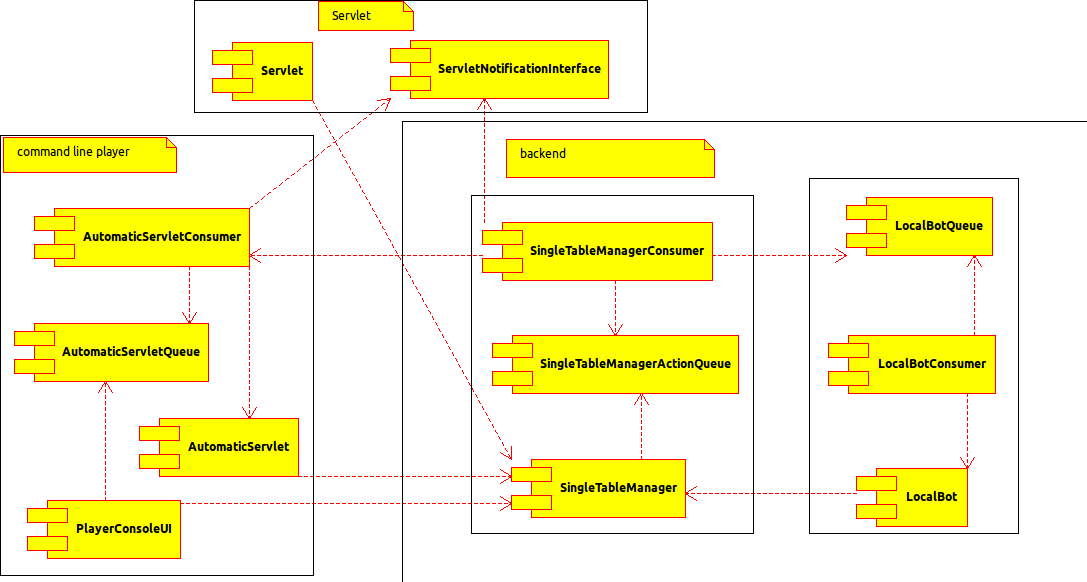
\includegraphics{backend_composit_structure.png}}
    \end{center}
    \caption{struttura composita di una parte di cupido}
    \label{fig:example}
  \end{figure}
\end{center}
\chapter{Iterazioni nel provesso di sviluppo}\section{Global table manager}
    In questa iterazione si \`e implementato il global table manager o gtm. Il gtm ha diverse responsabilit\'a: 
    \begin{description}
      \item[swarm]: 
	Gestire un insieme(chiamato in seguito swarm) di local table managers o ltm. In particolare gtm deve:
	\begin{itemize}
	  \item 
	    Permettere di aggiungere e rimuovere ltm dallo swarm.
	  \item
	    Controllare la consistenza dello swarm. A questo scopo fa polling degli ltm chiamando 	
	    \begin{verbatim} 
	      LocalTableManagerInterface.isAlive()
	    \end{verbatim}
	    ogni 
	    \begin{verbatim} 
	      GlobalTableManagerInterface.POLLING_DELAY
	    \end{verbatim} 
	    millisecondi.   
	  \item
	    Inoltrare le richieste delle servlet ad un ltm in modo da bilanciare il carico di lavoro tra gli ltm. A questo scopo gli ltm hanno associata una coppia di interi: il primo indica il numero di tavoli correntemente gestiti dall'ltm e il secondo indica il numero massimo di tavoli gestibili dall'ltm. Quando il gtm deve scegliere un ltm sul quale creare un nuovo tavolo, prende dallo swarm un ltm tra quelli che hanno un carico di lavoro pi\'u basso. Il carico di lavoro o workload di un ltm \`e definito come il rapporto tra i tavoli gestiti e il numero massimo di tavoli gestibili.
	\end{itemize}
	Ricapitolando lo swarm deve mantere associazioni tra interfacce ltm e coppie di interi, deve fornire operazioni di:
	\begin{itemize}
	   \item 	
	      Aggiunta con chiave una interfaccia ltm.
	   \item 
	      Rimozione con chiave una interfaccia ltm.
	   \item 
	      Modifica del numero di tavoli gestiti da un ltm.
	   \item 	
	      Scelta di un ltm con workload minimo.
	\end{itemize}
	Si \`e deciso di usare un ArrayList di record:
	\begin{verbatim}
	  interfaccia ltm, numero di tavoli gestiti, numero di tavoli gestibili
	\end{verbatim}
	Tale lista viene mantenuta ordinata con workload decrescente. Questa struttura dati minimizza il tempo di esecuzione dell'operazione pi\'u frequente cio\`e la scelta di un ltm.  Sia n il numero di ltm allora le complessit\'a in tempo al caso pessimo delle operazioni dello swarm sono:
	\begin{description}
	  \item[aggiunta]: 
	    O(n) perch\'e bisogna controllare che non ci siano due interfacce ltm uguali.
	  \item[rimozione]
	    O(n) perch\'e in questo caso non vengono confrontati i workload ma le interfacce.
	  \item[modifica]
	    O(n) perch\'e anche in questo caso non vengono confrontati i workload ma le interfacce.
	  \item[scelta]
	    O(log(n)) perch\'e: per scegliere un ltm con carico minimo basta prendere l'ultimo elemento della lista per\'o dopo bisogna incrementare il suo numero di tavoli gestiti e riordinare la lista.
	\end{description}
      \item[tables]:
	Mantenere alcune informazioni riguardo tutti i tavoli in Cupido. Tali informazioni sono tutte e sole quelle necessarie ad un giocatore che vuole unirsi ad una partita o che vuole vedere una partita e sono contenute nella classe 
	\begin{verbatim}
	  TableInfoForClient
	\end{verbatim}
	Ogni tavolo nel gmt \`e identificato da un descrittore di tavolo cio\`e una istanza di
	\begin{verbatim}
	  TableDescriptor
	\end{verbatim}
	Il gtm deve memorizzare associazioni tra descrittori di tavolo e informazioni del tavolo, inoltre deve avere a disposizione le operazioni di:
	\begin{itemize}
	  \item 
	    Aggiunta usando come chiave un descrittore di tavolo.
	  \item
	    Ricerca usando come chiave un descrittore di tavolo.
	  \item
	    Rimozione usando come chiave un descrittore di tavolo.
	  \item
	    Reperire una parte dei tavoli.
	\end{itemize}
	Si \`e scelto di memorizzare le informazioni dei tavoli in una 
      	\begin{verbatim}
	  LinkedHashMap<TableDescriptor, TableInfoForClient>
	\end{verbatim}
	L'hash \`e calcolato sui campi del descrittore del tavolo. In particolare il descrittore del tavolo contiene: una stringa che identifica un ltm, un intero che identifica il tavolo all'interno dell'ltm. In questo modo le prime tre operazioni richiedono tempo costante. La quarta operazione restituisce una quantit\'a di tavoli non superiore a
	\begin{verbatim}
	  GlobalTableManagerInterface.MAX_TABLE_LIST_SIZE
	\end{verbatim}
	I tavoli da restituire vengono copiati in una istanza di
	\begin{verbatim}
	  ArrayList<TableInfoForClient>
	\end{verbatim}
	e vengono scelti in modo casuale. In questo modo la dimensione dei dati inviati al client \`e costante. Al caso pessimo la complessit\'a in tempo di questa operazione \`e lineare nel numero di tavoli perch\'e per scegliere una parte dei valori da una tabella hash in modo uniformemente distribuito bisogna eventualmente iterare su tutti essi. Si \`e scelto di non fornire una operazione per reperire tutti i tavoli perch\'e il numero dei tavoli potrebbe essere troppo grande e quindi anche il traffico di rete conseguente. Un'altra strategia presa in considerazione \`e quella di un iteratore remoto ma \`e stata scartata perch\'e genera troppe chiamate remote e perch\'e la lista dei tavoli pu\'o cambiare tra due chiamate.
    \end{description}
  Gtm \`e usato attraverso RMI quindi il multithreading \`e gestito in automatico dalla JVM. La mutua eclusione sul gtm \`e gestita semplicemente usando metodi \begin{verbatim}
    synchronized
  \end{verbatim} 
  E' stata presa in considerazione un'altra strategia di mutua eclusione meno restrittiva cio\`e: tutte le operazioni hanno accesso esclusivo all gtm con l'eccezione che si permettono pi\'u operazioni in lettura allo stesso tempo. Tuttavia questa soluzione presenta il problema della starvation delle operazioni di scrittura quindi si \`e deciso di non adottarla.


\section{Local table manager}
  In questa iterazione si \`e implementato il local table manager o ltm. Ltm si occupa di una porzione dei tavoli di Cupido. In particolare ltm fornisce le operazioni seguenti:
  \begin{itemize}
    \item 
      Creare componenti table chiamate in seguito single table manager o stm.
    \item 
      Rimuovere un stm quando una partita finisce.
    \item 
      Cercare un stm quando un giocatore vuole unirsi ad una partita o guardare una partita.
  \end{itemize}
  Ltm mantiene in una tabella hash gli stm indicizzati da un intero che identifica l'stm in modo univoco nell'ltm. In questo modo le operazioni dell'ltm hanno complessit\'a in tempo costante.
  Per quanto riguarda il multithreading e la mutua eclusione valgono le stesse cose dette per il gtm.

\section{Gtm ed ltm console UI}
  In questa iterazione sono stati implementati due interpreti di comandi da console minimali per gtm ed ltm. I comandi forniti permettono di vedere lo stato interno del gtm e degli ltm. Quindi questi interpreti hanno una valenza per lo pi\'u in fase di debug e test. Potrebbero essere usati anche in un deploy reale per operazioni di manutenzione ma si \`e scelto di non farlo perch\'e non serve: in particolare non ci sono requisiti che vietano di riavviare il gtm o gli ltm in fase di esecuzione.

\section{Global chat}
  In questa iterazione \`e stata implementata la chat globale lato backend. La chat globale \`e un buffer di messaggi di dimensione 
  \begin{verbatim}
    GlobalChatInterface.MESSAGE_NUMBER
  \end{verbatim}
  Gli utenti di Cupido possono solo scrivere messaggi o reperire un certo numero di ultimi messaggi. Quindi i client fanno polling della chat globale e non ricevono notifiche quando un client invia un messaggio nella chat globale. Questo perch\'e si prevede la possibilit\'a di avere un numero elevato di utenti e quindi non conviene che la chat globale memorizzi un interfaccia di notifica per ognuno di essi e che invii notifiche a questa interfaccia ogni volta che arriva un nuovo messaggio nella chat globale.

\section{Database Manager}
  In questa iterazione \`e stata implementata la classe DatabaseManager che fornisce le operazioni descritte in SRS.


\section{Single table manager e logica del gioco}
  In questa iterazione \`e stato implementato stm. Stm si occupa di una singola partita. In particolare stm:
  \begin{itemize}
    \item 
      gestisce giocatori e bot: permette ad un giocatore di unirsi alla partita  di lasciare la partita e di giocare, permette al creatore del tavolo di aggiungere bot, sostituisce un giocatore con un bot se questo lascia la partita dopo l'inizio, notifica i giocatori di quello che succede nella partita.
    \item
      gestisce i visitatori: permette ad un visitatore di aggiungersi alla partita o di lasciare la partita, invia ai visitatori le notifiche di quello che succede nella partita.
    \item
      gestisce le carte: da le carte e controlla che le mosse dei giocatori siano valide.
    \item
      gestisce i punteggi dei giocatori.
  \end{itemize}
  

\section{Local Bot}
  In questa iterazione \`e stato implementato un bot, cio\`e un giocatore automatico. Quando il bot riceve le carte, le ordina dalla pi\'u alta alla pi\'u bassa e poi in base al seme. Quando deve passare le carte sceglie le prime tre che ha. Quando deve giocare una carta sceglie la prima carta valida che ha.

\section{Command line player}
  In questa iterazione \`e stato implementato un interprete di comandi testuale per un utente di Cupido. L'interprete fornisce una ampia gamma di comandi: creare un tavolo, ottenere la lista di tutti i tavoli, unirsi ad una partita, vedere una partita e giocare una partita. Per una descrizione dei comandi si veda la documentazione della classe
  \begin{verbatim}
    PlayerConsoleUI
  \end{verbatim}
  I comandi possono essere presi da console o da un file di input. Usando un file di input si pu\'o far giocare una partita a degli utenti in modo completamente automatico.

\section{Ristrutturazione della comunicazione e della mutua esclusione}
  In questa iterazione \`e stata re-implementata la comunicazione fra le varie
  componenti del backend per evitare deadlock.

  In particolare, all'inizio di questa iterazione tutte le notifiche venivano
  inviate in modo sincrono tramite RMI, e all'arrivo di una notifica, essa
  veniva gestita direttamente nel metodo chiamato attraverso RMI. Questo
  significa che, ad esempio, quando una servlet chiamava con RMI un metodo
  del tavolo, esso inviava le notifiche relative ed aspettava che fossero
  gestite prima di restituire il controllo alla servlet.

  Questa implementazione dava vari problemi: le servlet non potevano chiamare
  metodi del tavolo durante la gestione di una notifica (perch\'e i metodi
  del tavolo sono synchronized e si sarebbe creato un deadlock).
  Inoltre, quando una servlet chiamava un metodo del tavolo, il tavolo non
  poteva notificare la stessa servlet, perch\'e questo avrebbe causato
  problemi di concorrenza all'interno della servlet.

  Per risolvere questi problemi, \`e stata aggiunta una ActionQueue ai tavoli
  e ai bot, per gestire rispettivamente le notifiche in uscita e in ingresso.

  ActionQueue \`e una classe creata durante questa iterazione. Questa classe
  supporta l'accodamento di azioni e le esegue in un secondo momento, in un
  thread dedicato.

  Ogni tavolo ora usa una ActionQueue per le notifiche in uscita:
  al posto di inviare le notifiche alle servlet (o ai bot) direttamente, esse
  vengono accodate nella ActionQueue ed eseguite dopo aver restituito il
  controllo alla servlet (o al bot).

  I bot usano anch'essi una ActionQueue, ma per le notifiche in entrata:
  in questo modo, quando l'ActionQueue del tavolo invia le notifiche, non
  deve aspettare che esse vengano gestite dai bot, cosa che potrebbe
  comportare delle chiamate al tavolo da parte dei bot (ad esempio, quando
  il bot deve giocare una carta).
  Il diagramma di struttura composita della parte del backend che gesiste una 
  partita \`e in figura \ref{fig:struttura composita di stm}.

\begin{figure}
  \begin{center}
    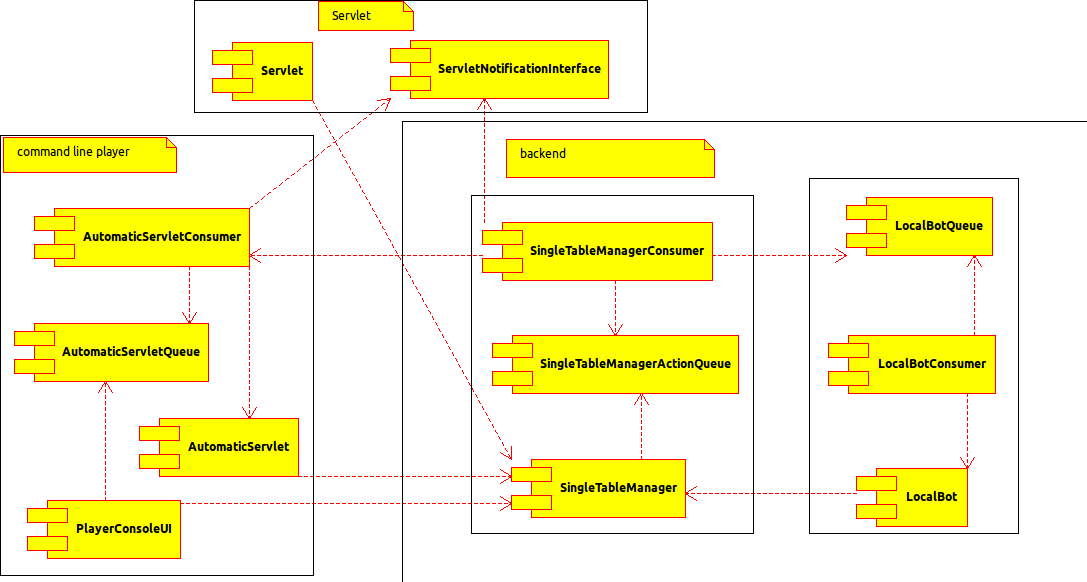
\includegraphics[scale=0.5]{backend_composit_structure.png}  
  \end{center}
  \caption{Struttura composita di stm}
  \label{fig:struttura composita di stm}
\end{figure}

\section{Test del solo backend}
  La cartella cupiboBackendImpl/test contiene i file per i test automatici del backend. Sono stati eseguiti i seguenti cinque test automatici sul backend:
  \begin{itemize}
    \item 
      Un giocatore crea un tavolo, aggiunge tre bot e gioca. Questo test si esegue con il comando
      \begin{verbatim}
	./cupidoBackendImpl/test/test1
      \end{verbatim}
      il quale esegue un giocatore a riga di comando che legge i comandi dal file 
      \begin{verbatim}
	./cupidoBackendImpl/test/createTableAndAddThreeBot
      \end{verbatim}
    \item
      Un giocatore crae un tavolo e aggiungie due bot, in seguito un altro giocatore si unisce alla partita. Questo test si esegue con il comando
      \begin{verbatim}
	./cupidoBackendImpl/test/test2
      \end{verbatim}
      il quale esegue due giocatori a riga di comando che leggono i comandi dai file:
      \begin{verbatim}
	./cupidoBackendImpl/test/createTableAndAddTwoBot, ./cupidoBackendImpl/test/joinATable
      \end{verbatim}
    \item
      Un giocatore crea un tavolo, aggiunge tre bot e gioca, nel frattempo un visitatore guarda la partita. Questo test si esegue con il comando
      \begin{verbatim}
	./cupidoBackendImpl/test/test3
      \end{verbatim}
      il quale esegue un giocatore come nel primo test e in pi\'u esegue un visitatore da riga di comando che legge i comandi dal file
      \begin{verbatim}
	./cupidoBackendImpl/test/view
      \end{verbatim}
    \item
      Un giocatore crea un tavolo, aggiunge tre bot, gioca per un po e poi abbanona la partita. Questo test si esegue con il comando
      \begin{verbatim}
	./cupidoBackendImpl/test/test4
      \end{verbatim}
      il quale esegue un visitatore ed un giocatore da riga di comandi che legge i comandi dal file 
      \begin{verbatim}
	./cupidoBackendImpl/test/createTableAndAddThreeBotLeave
      \end{verbatim}
    \item
      Un giocatore crea un tavolo e aggiunge due bot, nel frattempo un altro giocatore si unisce alla partita e in seguito i due giocatori giocano. Dopo qualche turno il giocatore non creatore lascia la partita e viene rimpiazzato da un bot. Questo test si esegue con il comando
      \begin{verbatim}
	./cupidoBackendImpl/test/test5
      \end{verbatim}
  \end{itemize}
  Tutti i test sono andati a buon fine.
\chapter{Test del backend}\input{test}

\printindex

\end{document}
